\section{Intelligent agents}
\label{sec:agents}

\subsection{Rational agents}
\label{sec:agents-rational}

\begin{definition}[Rational agent]
\label{def:rational}
``For each possible percept sequence, a rational agent should select an action that is expected to maximize its performance measure, given the evidence provided by the percept sequence and whatever built-in knowledge the agent has'' \citep[\S2.2.2]{russell2020aima}.
\end{definition}

The definition uses three terms we fix first. An agent is anything that perceives its
environment through sensors and acts on it through actuators \citep[\S2.1]{russell2020aima}; a
software agent's sensors deliver file contents and network input, and its actuators write files
and send output. A \emph{percept} is the content the sensors deliver at one instant, and the
\emph{percept sequence} is the complete history of everything the agent has perceived. The
agent's behavior is described by its \emph{agent function}, which maps any percept sequence to
an action, and an agent's choice may depend on that sequence and its built-in knowledge but on
nothing it has not perceived \citep[\S2.1]{russell2020aima}. A \emph{performance measure}
evaluates the sequence of environment states the agent's actions bring about
\citep[\S2.2.1]{russell2020aima}: it scores the environment, not the agent's beliefs about it.
One more distinction carries the rest of these notes. The agent function is an abstract
description of behavior, while the \emph{agent program} is the concrete implementation that
computes it, running on an architecture that makes percepts available and carries out the
actions the program chooses \citep[\S2.1, \S2.4]{russell2020aima}. We fix the function when we
specify the task, and the program is where our design choices live.

\begin{figure}[htbp]
  \centering
  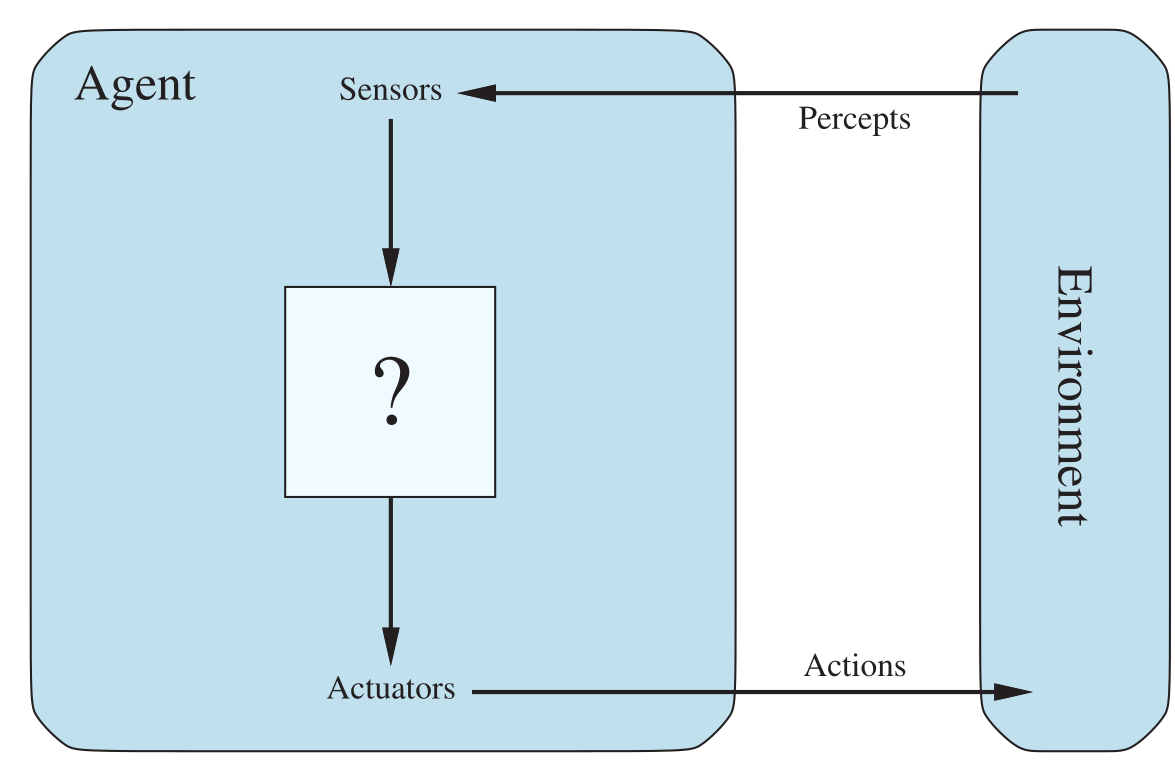
\includegraphics[width=\linewidth]{figures/aima-fig2-1.png}
  \caption{An agent and its environment. Figure~2.1 of \citet{russell2020aima}, reproduced from
  the Global Edition (\copyright~Pearson Education Limited 2022).}
  \label{fig:agents-fig21}
\end{figure}

What is rational at any given time depends on four things \citep[\S2.2.2]{russell2020aima}:
\begin{itemize}
  \item the performance measure that defines the criterion of success;
  \item the agent's prior knowledge of the environment;
  \item the actions that the agent can perform;
  \item the agent's percept sequence to date.
\end{itemize}

\subsubsection{The running example: \msa{}}
\msa{} is the agent we build through five versions in this block. Its environment is one
application, OWASP BenchmarkPython at a pinned commit \citep{owasp-benchmarkpython}, together
with the alerts a static scanner reports against it. It takes one alert at a time, reads the
alert as an issue report, localizes the code the alert names, edits that code, and submits a
patch. \Cref{fig:agents-state} is the whole agent: three states and five transitions, with each
label read as an event and then a condition in brackets.
\begin{itemize}
  \item \textbf{Controller} decides the next action.
  \item \textbf{Tool} executes the action the controller requested and hands back an
  observation. There is one node per tool, and this version has three: \demoref{read\_file} over
  a range of lines, \demoref{search} for a pattern, and \demoref{edit} as a replacement in one
  file that the runtime applies to the working tree.
  \item \textbf{Submit} validates the submission. On \emph{accepted} the run ends. On
  \emph{rejected} the feedback goes back to the controller, which may act again.
\end{itemize}
Every version in this block is a change to that machine: a state, an edge, or a different
component deciding. Nothing else about the agent changes.

\begin{figure}[htbp]
  \centering
  \begin{adjustbox}{width=\linewidth}% The state machine of mini-swe-agent: three states, five transitions.
% Labels read as event, then condition in brackets.
\begin{tikzpicture}[x=1cm, y=1cm,
  st/.style={gnode, align=center, minimum width=4.1cm, minimum height=1.45cm, inner sep=3pt},
  ctrl/.style={st, fill=ibmblue!12},
  tool/.style={st, fill=black!6},
  subm/.style={st, fill=ibmfg!7},
  ghost/.style={draw=ibmfg!35, rounded corners=2pt, fill=white, line width=0.4pt,
                minimum width=4.1cm, minimum height=1.45cm},
  fl/.style={-{Stealth[length=2.4mm]}, thick, draw=ibmfg!85},
  ev/.style={font=\sffamily\footnotesize, align=center, inner sep=2.5pt, fill=white},
  note/.style={font=\sffamily\scriptsize, align=center, inner sep=2pt, text=ibmfg!70}]
  \def\cond#1{\\[-1pt]{\scriptsize\color{ibmfg!70}#1}}

  \node[circle, fill=ibmfg, inner sep=2.4pt] (start) at (-0.4,0) {};
  \node[font=\sffamily\footnotesize\bfseries, above=3pt of start] {Start};
  \node[ghost] (t2) at (10.4,0.18) {};
  \node[ghost] (t1) at (10.3,0.09) {};
  \node[tool]  (tool) at (10.2,0) {\textbf{Tool}\cond{execute the requested tool}};
  \node[note, above=8pt of t2] {one node per tool: read, search, edit};
  \node[ctrl] (ctrl) at (3.4,0) {\textbf{Controller}\cond{decide the next action}};
  \node[subm] (sub)  at (3.4,-3.35) {\textbf{Submit}\cond{validate the submission}};
  \node[circle, draw=ibmfg, thick, inner sep=3.2pt] (end) at (3.4,-5.85)
        {\tikz\node[circle, fill=ibmfg, inner sep=2.2pt]{};};
  \node[font=\sffamily\footnotesize\bfseries, below=3pt of end] {End};

  \draw[fl] (start) -- (ctrl);
  \draw[fl] (ctrl.east) -- node[ev, above=1pt]{tool requested\cond{[tool\_name, args]}} (tool.west);
  \draw[fl] (tool.south) to[out=-90, in=-20, looseness=0.75]
            node[ev, pos=0.52]{tool finished\cond{[observation]}} (ctrl.south east);
  \draw[fl] (ctrl.south) -- node[ev, left=1pt, pos=0.52]{submission requested\cond{[patch]}} (sub.north);
  \draw[fl] (sub.west) to[out=178, in=192, looseness=1.7]
            node[ev, left=2pt, pos=0.5]{rejected\cond{[feedback]}} (ctrl.south west);
  \draw[fl] (sub.south) -- node[ev, right=3pt]{accepted} (end.north);
\end{tikzpicture}
\end{adjustbox}
  \caption{\msa{} as a state machine. Blue is the state where a model call decides, grey is
  runtime-owned. The run ends only when a submission is accepted.}
  \label{fig:agents-state}
\end{figure}

One alert serves as the worked example throughout: Bandit's rule B608, string-based SQL query
construction, at line~46 of \path{testcode/BenchmarkTest00283.py}. Line~46 builds the query by
interpolating the request value \demoref{bar} into the string, and line~49 executes it. The
patch is two lines in one file, a placeholder in the query and \demoref{bar} bound when the
query runs.

\begin{lstlisting}[caption={The worked alert, before and after. Two lines in one file.},label=lst:agents-patch]
# before: the value is interpolated into the query text
sql = f'SELECT username from USERS where password = \'{bar}\''
cur.execute(sql)

# after: the query carries a placeholder and the value is bound
sql = 'SELECT username from USERS where password = ?'
cur.execute(sql, (bar,))
\end{lstlisting}

One very simple agent function is the following. If the alert names a location that is not yet
in the percept sequence, read it. If the code has been read but not edited, edit it. Once the
edit is applied, submit. \Cref{fig:agents-sequence} traces that function on the worked alert.
A full tabulation of it would be unbounded unless the budget bounds the percept sequence.

\begin{figure}[htbp]
  \centering
  \begin{adjustbox}{width=\linewidth}% One run of mini-swe-agent on the worked alert. Actions left to right, percepts right to left.
\begin{tikzpicture}[x=1cm, y=1cm,
  head/.style={gnode, minimum width=3.4cm, font=\sffamily\small},
  life/.style={draw=black!45, dashed},
  act/.style={-{Stealth[length=2.6mm]}, line width=1.4pt, draw=ibmblue},
  per/.style={-{Stealth[length=2.6mm]}, line width=1.4pt, draw=red!70!black},
  msg/.style={font=\sffamily\footnotesize, fill=white, inner sep=1.5pt, align=center}]
  \node[head] (agent) at (0,0) {Controller};
  \node[head] (rt) at (11.4,0) {Runtime and tools};
  \draw[life] (agent.south) -- (0,-7.4);
  \draw[life] (rt.south) -- (11.4,-7.4);
  \draw[per] (11.4,-1.0) -- (0,-1.0) node[msg, midway, above]
        {alert as an issue report: Bandit B608,\\ \texttt{testcode/BenchmarkTest00283.py} line 46};
  \draw[act] (0,-2.0) -- (11.4,-2.0) node[msg, midway, above] {\texttt{read\_file(testcode/BenchmarkTest00283.py, 40--52)}};
  \draw[per] (11.4,-3.1) -- (0,-3.1) node[msg, midway, above]
        {line 46 builds the query from \texttt{bar} with an f-string;\\ line 49 runs \texttt{cur.execute(sql)}};
  \draw[act] (0,-4.1) -- (11.4,-4.1) node[msg, midway, above] {\texttt{edit}: a placeholder on line 46, \texttt{bar} bound on line 49};
  \draw[per] (11.4,-5.0) -- (0,-5.0) node[msg, midway, above] {edit applied: two lines changed};
  \draw[act] (0,-5.9) -- (11.4,-5.9) node[msg, midway, above] {\texttt{submit}: the patch, one file, two lines};
  \draw[per] (11.4,-6.9) -- (0,-6.9) node[msg, midway, above]
        {accepted: the patch applies and the rescan\\ no longer reports line 46. The run ends};
\end{tikzpicture}
\end{adjustbox}
  \caption{One run on the worked alert. Blue arrows are actions the controller requests; red
  arrows are percepts the runtime returns.}
  \label{fig:agents-sequence}
\end{figure}

\demoref{search} does not appear in that run, because the alert names the line and the value it
interpolates is assigned in the same function. It earns its place as soon as the fix has to
touch code the alert does not name, which is the case \cref{sec:agents-rational-limits} turns
on.

\subsubsection{Is this a rational agent?}
\label{sec:agents-rational-limits}
That depends. We have to say what the performance measure is, what is known about the
environment, and what the agent can do and perceive. Assume the following.
\begin{itemize}
  \item The performance measure awards one point if the submitted patch removes the weakness the
  alert reports and leaves the endpoint behaving as it did, over a lifetime of one alert.
  \item The geography of the environment is known a priori: the application's layout and the
  behavior of the tools. A read returns the lines of the working tree, a search returns every
  location that matches, and an edit replaces text in one file. Which change removes the
  weakness is not known.
  \item The only available actions are \demoref{read\_file}, \demoref{search}, \demoref{edit},
  and \demoref{submit}.
  \item The agent correctly perceives what its tools return.
\end{itemize}
Under these circumstances the agent is rational: reading the flagged lines before editing them
is the action that maximizes expected performance, and no other agent does better in
expectation.

The measure and the check are not the same thing, and the gap is worth naming now. The Submit
state can establish that the patch applies, that it touches the line the alert named, and that a
rescan no longer reports it. None of that establishes that the endpoint still returns what it
returned before. Accepted is not correct, and \cref{sec:validation} is where that distinction
becomes a component.

The same agent is irrational under different circumstances. If the performance measure charges
a point for each tool call, an agent that reads whole files fares poorly, and a better agent
reads the smallest range that answers its question. If the value the query interpolates arrives
from a helper in another file, an agent that edits only the flagged line can leave the weakness
in place or change what the endpoint returns. A better agent searches for the helper first, and
how far to follow the value is the depth of investigation we fix. And once the edit is applied
and accepted, an agent that keeps editing wastes every further call and risks breaking
behavior; a better agent submits as soon as it is sure. Those three circumstances are the
budget, the depth of investigation, and termination, and each later section makes one of them a
decision.

\begin{foodforthought}
What are your yardsticks for the agent you are developing, and why? Before you write a node,
write down its performance measure, the depth of investigation you will allow, and the rule
that ends an investigation, and say for each what it rewards and what it lets through.
\end{foodforthought}

Three consequences of the definition matter for what follows \citep[\S2.2.3]{russell2020aima}.
Rationality is not omniscience: it maximizes expected performance, not actual performance, and
the agent cannot know whether its edit removes the weakness before it has read the code around
the alert. Acting to change future percepts, information gathering, is part of rationality and
not a detour: our agent reads the flagged function before it edits because looking is how it
maximizes expected performance. And an agent that relies on its designer's prior knowledge
rather than on its own percepts lacks autonomy. A fixed workflow, whose sequence of read, edit,
and submit steps we write in advance, is the extreme of that dependence, and it is where
\cref{sec:fixed} starts.

\subsection{The task environment}
\label{sec:agents-environment}

\begin{definition}[Task environment and PEAS]
\label{def:peas}
The performance measure, the environment, the actuators, and the sensors together form the
\emph{task environment}, written as a PEAS description. ``In designing an agent, the first step must always be to specify the task environment as fully as possible'' \citep[\S2.3.1]{russell2020aima}.
\end{definition}

Task environments are the problems to which rational agents are the solutions, and the nature of
the task environment decides the appropriate design for the agent program
\citep[\S2.3]{russell2020aima}. \Cref{tab:agents-peas} is the PEAS description of \msa{}.

\begin{table*}[tbp]
  \caption{PEAS description of the task environment for \msa{}.}
  \label{tab:agents-peas}
  \begin{adjustbox}{width=\linewidth}\begin{tabularx}{\linewidth}{XXXX}
    \toprule
    Performance measure & Environment & Actuators & Sensors \\
    \midrule
    The weakness the alert reports is gone and the endpoint still returns what it returned before; bounded cost in tool calls and tokens & OWASP BenchmarkPython at a pinned commit; one alert from a static scanner, read as an issue report; the working tree the agent edits & \demoref{read\_file(path, range)}, \demoref{search(pattern)}, \demoref{edit(path, old, new)}, \demoref{submit(patch)} & The alert; file excerpts; search hits; edit confirmations; the validation result; tool errors \\
    \bottomrule
  \end{tabularx}\end{adjustbox}
\end{table*}

The environment is not the whole world but the part whose state we care about when we design
the agent: what affects what it perceives, and what its actions affect
\citep[\S2.1]{russell2020aima}. Nothing outside the working tree and the alert affects what
our agent perceives, and its actions affect nothing outside the working tree. The last column is
the narrow part: every percept after the first arrives as the result of a tool call.

\subsection{Properties of task environments}
\label{sec:agents-properties}

Task environments vary along seven dimensions, and the dimensions decide, to a large extent,
which agent designs and which families of techniques apply \citep[\S2.3.2]{russell2020aima}.
Each table below gives one pair: the defining sentence and the standard examples
\citep[Fig.~2.6]{russell2020aima}.

\subsubsection{Fully observable vs.\ partially observable}
\begin{center}
\begin{adjustbox}{width=\linewidth}\begin{tabularx}{\linewidth}{L{0.18\linewidth}XX}
  \toprule
  & Fully observable & Partially observable \\
  \midrule
  Definition & ``If an agent's sensors give it access to the complete state of the environment at each point in time, then we say the task environment is fully observable.'' Effectively fully observable if the sensors detect every aspect relevant to the choice of action. & Sensors are noisy or inaccurate, or parts of the state are missing from the sensor data. With no sensors at all, unobservable. \\
  Examples & Crossword, chess with a clock, backgammon, image analysis & Poker, taxi driving, medical diagnosis, part-picking robot, refinery controller \\
  \bottomrule
\end{tabularx}\end{adjustbox}
\end{center}

\subsubsection{Single-agent vs.\ multiagent}
\begin{center}
\begin{adjustbox}{width=\linewidth}\begin{tabularx}{\linewidth}{L{0.18\linewidth}XX}
  \toprule
  & Single-agent & Multiagent \\
  \midrule
  Definition & No other entity's behavior is best described as maximizing a performance measure whose value depends on this agent's behavior. & ``The key distinction is whether B's behavior is best described as maximizing a performance measure whose value depends on agent A's behavior.'' Competitive (chess) or partially cooperative (taxi driving). \\
  Examples & Crossword, medical diagnosis, image analysis, part-picking robot, refinery controller & Chess with a clock, poker, backgammon, taxi driving, English tutor \\
  \bottomrule
\end{tabularx}\end{adjustbox}
\end{center}

\subsubsection{Deterministic vs.\ nondeterministic}
\begin{center}
\begin{adjustbox}{width=\linewidth}\begin{tabularx}{\linewidth}{L{0.18\linewidth}XX}
  \toprule
  & Deterministic & Nondeterministic \\
  \midrule
  Definition & ``If the next state of the environment is completely determined by the current state and the action executed by the agent(s), then we say the environment is deterministic.'' & Otherwise. A partially observable environment can appear nondeterministic. \emph{Stochastic} is reserved for models that quantify the possibilities with probabilities. \\
  Examples & Crossword, chess with a clock, image analysis & Poker, backgammon, taxi driving, medical diagnosis, refinery controller (listed as stochastic) \\
  \bottomrule
\end{tabularx}\end{adjustbox}
\end{center}

\subsubsection{Episodic vs.\ sequential}
\begin{center}
\begin{adjustbox}{width=\linewidth}\begin{tabularx}{\linewidth}{L{0.18\linewidth}XX}
  \toprule
  & Episodic & Sequential \\
  \midrule
  Definition & ``In an episodic task environment, the agent's experience is divided into atomic episodes. In each episode the agent receives a percept and then performs a single action. Crucially, the next episode does not depend on the actions taken in previous episodes.'' & ``In sequential environments, on the other hand, the current decision could affect all future decisions.'' \\
  Examples & Image analysis, part-picking robot & Crossword, chess, poker, backgammon, taxi driving, medical diagnosis, refinery controller, English tutor \\
  \bottomrule
\end{tabularx}\end{adjustbox}
\end{center}

\subsubsection{Static vs.\ dynamic}
\begin{center}
\begin{adjustbox}{width=\linewidth}\begin{tabularx}{\linewidth}{L{0.18\linewidth}XX}
  \toprule
  & Static & Dynamic \\
  \midrule
  Definition & The environment cannot change while the agent is deliberating. The agent need not keep looking at the world while deciding, nor worry about the passage of time. & ``If the environment can change while an agent is deliberating, then we say the environment is dynamic for that agent.'' \emph{Semidynamic} if the environment does not change with time but the performance score does. \\
  Examples & Crossword, poker, backgammon; chess with a clock and image analysis are semidynamic & Taxi driving, medical diagnosis, part-picking robot, refinery controller, English tutor \\
  \bottomrule
\end{tabularx}\end{adjustbox}
\end{center}

\subsubsection{Discrete vs.\ continuous}
\begin{center}
\begin{adjustbox}{width=\linewidth}\begin{tabularx}{\linewidth}{L{0.18\linewidth}XX}
  \toprule
  & Discrete & Continuous \\
  \midrule
  Definition & ``The discrete/continuous distinction applies to the state of the environment, to the way time is handled, and to the percepts and actions of the agent.'' A finite number of distinct states, percepts, and actions. & State, time, percepts, or actions sweep through a range of values. \\
  Examples & Crossword, chess with a clock, poker, backgammon, English tutor & Taxi driving, medical diagnosis, image analysis, part-picking robot, refinery controller \\
  \bottomrule
\end{tabularx}\end{adjustbox}
\end{center}

\subsubsection{Known vs.\ unknown}
\begin{center}
\begin{adjustbox}{width=\linewidth}\begin{tabularx}{\linewidth}{L{0.18\linewidth}XX}
  \toprule
  & Known & Unknown \\
  \midrule
  Definition & ``In a known environment, the outcomes (or outcome probabilities if the environment is nondeterministic) for all actions are given.'' The distinction concerns the agent's knowledge of the laws of the environment, not the environment itself. & The agent has to learn how the environment works before it can decide well. A new video game may show the whole screen and still not say what the buttons do. \\
  Examples & Chess and poker: the rules can be supplied in full & Driving a rented car in a new country \\
  \bottomrule
\end{tabularx}\end{adjustbox}
\end{center}

The hardest case \citep[\S2.3.2]{russell2020aima} is partially observable, multiagent,
nondeterministic, sequential, dynamic, continuous, and unknown. The task environment of \msa{} is
partially observable, single-agent, deterministic, sequential within one alert and episodic
across alerts, static, discrete, and known: it shares two properties with the hardest case,
partial observability and sequentiality, and none of the other five. Partial observability alone is what makes the task an
investigation, and it is the property every later section responds to.

\subsection{Where the vocabulary lives in \msa{}}
\label{sec:agents-mapping}

Every term defined above corresponds to something \msa{} actually contains, with one exception:
the agent function is an abstract description of behavior and has no counterpart in the source.
\Cref{tab:agents-mapping} gives the correspondence, and \cref{fig:agents-annotated} writes the
same names onto the machine itself.

Two of those correspondences do the most work. The agent program is not one component but two: the
controller, which proposes the next action, and the runtime's control loop, which executes it,
updates state, routes, and stops. Beneath both sits the architecture, which is not part of the
program at all but the process the run lives in, the model client the controller calls, and the
tool implementations that turn a requested action into a real one. Every version that follows,
from the chain to the reflection step, changes what the controller is asked to decide, and none of
them changes who executes. Working
state is the second: it holds what the agent has seen so far, and how that record is declared and
updated is taken up in Part~B.

% Not a float: this figure and the table below it are read against each other, so they must not
% drift apart.
\begin{center}
  \begin{adjustbox}{width=\linewidth}% The state machine of mini-swe-agent with the vocabulary named on it, so each label can be read
% against the mapping table. Channels are kept apart: submit runs down the right, rejected up the left.
\begin{tikzpicture}[x=1cm, y=1cm,
  st/.style={gnode, align=center, minimum width=3.6cm, minimum height=1.3cm, inner sep=3pt},
  ctrl/.style={st, fill=ibmblue!12},
  rt/.style={st, fill=black!6},
  tool/.style={draw=ibmfg!60, rounded corners=2pt, fill=white, align=center,
               minimum width=4.1cm, minimum height=0.95cm, inner sep=3pt, font=\sffamily\footnotesize},
  fl/.style={-{Stealth[length=2.4mm]}, thick, draw=ibmfg!85},
  dotted/.style={-{Stealth[length=1.8mm]}, draw=ibmfg!50, densely dotted, line width=0.6pt},
  ev/.style={font=\sffamily\scriptsize, align=center, inner sep=2pt, fill=white},
  tag/.style={font=\sffamily\scriptsize\bfseries, text=ibmblue, inner sep=2pt},
  sub/.style={font=\sffamily\scriptsize, text=ibmfg!65, align=left, inner sep=2pt}]

  \def\cond#1{\\[-1pt]{\scriptsize\color{ibmfg!65}#1}}

  % the environment encloses the agent and the tools that reach into it
  \draw[draw=ibmfg!45, dashed, thick, rounded corners=8pt] (-1.6,3.15) rectangle (17.5,-7.5);
  \node[tag, anchor=north west] at (-1.45,3.05) {Environment};
  \node[sub, anchor=north west] at (-1.45,2.68) {the working tree at the pinned commit, and the alert};

  % the agent program: the part that decides, and the part that executes
  \draw[draw=ibmfg!80, thick, rounded corners=6pt] (-1.0,2.05) rectangle (7.9,-6.9);
  \node[tag, anchor=north west] at (-0.85,1.95) {Agent program};

  \node[circle, fill=ibmfg, inner sep=2.2pt] (start) at (3.4,1.45) {};
  \node[font=\sffamily\scriptsize\bfseries, right=3pt of start] {Start};

  \node[ctrl] (ctrl)  at (3.4,0.1)  {\textbf{Controller}\cond{decide the next action}};
  \node[rt]   (state) at (3.4,-2.6) {\textbf{Working state}\cond{locations, excerpts, edits, cost}};
  \node[rt]   (sub)   at (3.4,-5.4) {\textbf{Submit}\cond{validate the submission}};
  \node[circle, draw=ibmfg, thick, inner sep=3.0pt] (end) at (10.4,-5.4)
        {\tikz\node[circle, fill=ibmfg, inner sep=2.0pt]{};};
  \node[font=\sffamily\scriptsize\bfseries, above=2pt of end] {End};

  \draw[fl] (start) -- (ctrl);
  \draw[{Stealth[length=2.4mm]}-{Stealth[length=2.4mm]}, thick, draw=ibmfg!85]
        (ctrl) -- node[ev, right=1pt]{read, update} (state);
  \node[tag, anchor=north] at (3.4,-3.42) {Working state};

  % one node per tool, staggered, reached by dotted lines from the single request edge
  \node[tool] (t1) at (13.0,1.75)  {\demoref{read\_file(path, range)}};
  \node[tool] (t2) at (13.4,0.45)  {\demoref{search(pattern)}};
  \node[tool] (t3) at (13.8,-0.85) {\demoref{edit(path, old, new)}};
  \coordinate (hub) at (10.0,0.65);

  \draw[fl] ([yshift=4.5mm]ctrl.east) -- node[ev, above=1pt]{action\cond{[tool\_name, args]}} (hub);
  \node[tag, anchor=south] at (6.6,1.15) {Actions};
  \draw[dotted] (hub) -- (t1.west);
  \draw[dotted] (hub) -- (t2.west);
  \draw[dotted] (hub) -- (t3.west);

  \draw[fl] (t3.south) to[out=-90, in=-12, looseness=0.6]
        node[ev, pos=0.62]{percept\cond{[observation]}} ([yshift=-3.5mm]ctrl.east);
  \node[tag, anchor=north west] at (8.75,-0.5) {Percepts};

  \node[tag, anchor=north west] at (11.2,-2.35) {Architecture};
  \node[sub, anchor=north west] at (11.2,-2.75)
        {the process, the model client,\\ and the code behind each tool};

  % submit runs down the right of the column, rejected comes back up the left
  \draw[fl] (ctrl.east) -- (6.6,0.1) -- (6.6,-4.3)
        node[ev, pos=0.62]{submit\cond{[patch]}} -- (3.4,-4.3) -- (sub.north);
  \draw[fl] (sub.west) -- ++(-1.9,0) coordinate (l1) |- (ctrl.west)
        node[ev, pos=0.72, above]{rejected\cond{[feedback]}};
  \draw[fl] (sub.east) -- node[ev, midway, above]{accepted} (end.west);

  \node[tag, anchor=north west] at (8.6,-6.0) {Performance measure};
  \node[sub, anchor=north west] at (8.6,-6.4)
        {the Submit checks, and the four token counters};
\end{tikzpicture}
\end{adjustbox}
  \captionof{figure}{The same machine as \cref{fig:agents-state}, with the vocabulary named on it.
  The dashed box is the environment, the solid box is the agent program, and the three tools are the
  only path between them. Each blue label names a row of \cref{tab:agents-mapping}.}
  \label{fig:agents-annotated}
\end{center}

\begin{table}[htbp]
  \caption{The vocabulary mapped onto the components every version shares.}
  \label{tab:agents-mapping}
  \begin{adjustbox}{width=\linewidth}\begin{tabularx}{\linewidth}{L{0.25\linewidth}XX}
    \toprule
    Concept & In \msa{} & Where it appears in the demo source \\
    \midrule
    Performance measure & A patch that removes the weakness and leaves behavior unchanged, at bounded cost & The Submit state's checks in the trace and the trace's four token counters \\
    Environment & The working tree at the pinned commit and the alert & The task record: repository, commit, rule, file, line \\
    Percepts & The alert; excerpts, search hits, edit confirmations, the validation result, tool errors & Tool-result events in the trace \\
    Actions & \demoref{read\_file}, \demoref{search}, \demoref{edit}, \demoref{submit} & The three tool signatures and the submit transition \\
    Working state & Locations found, excerpts read, edits applied, cost, status & The state schema: a typed record with one reducer per field \\
    Agent program & Controller: decides the next action. The runtime's control loop: executes it, updates state, routes, and stops & The controller node; the dispatcher, the reducers, the routing predicate, the terminal statuses \\
    Architecture & The process the run lives in, the model client, and the tool implementations & The process the demo starts, the client behind the controller node, and the code behind the tool layer \\
    \bottomrule
  \end{tabularx}\end{adjustbox}
\end{table}

\begin{demostub}
Insert (1) the state schema of the reactive loop as declared in the demo source, with its
reducers named, and
(2) the three tool signatures, so that every row of \cref{tab:agents-mapping} can be read against
the code it names.
\end{demostub}

\subsection{Exercises}

\begin{enumerate}
  \item The performance measure in \cref{tab:agents-peas} asks that the endpoint still behave as
  it did, and the Submit state cannot check that. Write a check that would, name the tool it
  needs, and say what it would add to the cost of every alert.
  \item Consider \msa{} on the worked alert. Name an action it can take that is rational under
  Definition~\ref{def:rational} and yet changes nothing in the working tree, and say what it
  changes instead.
  \item Extend \cref{fig:agents-sequence} with the run in which the value the query interpolates
  arrives from a helper in another file. At which step does the simple agent function stop being
  rational, and what must the agent's internal state hold for it to reach the helper?
  \item Pick any row of \cref{tab:agents-mapping} and name the trace event that would let you
  check, after a run, that the component did what the row says. Which row has no such event, and
  what would you add to the trace to get one?
\end{enumerate}

\subsection{Reading}

\citet{russell2020aima}, \S2.3.2 (properties of task environments) and
\S\S2.4.1--2.4.5 (agent programs through utility-based agents). The agent programs of \S2.4 are
taken up in \cref{sec:patterns}, once the five versions exist to place on them.
Covered in these notes only: \S2.1, \S2.2, and \S2.3.1. The state representations of \S2.4.7 are
taken up in Part~B with the state.

\paragraph{Looking ahead.}
The rest of these notes walk the question one decision at a time, on \msa{}, each version a
runnable program rather than a diagram. A \emph{fixed workflow} (\cref{sec:fixed}) makes every
control decision at design time and lets the model fill in content. It is an agent without
autonomy, rational only while the designer's prior knowledge holds, and Agentless
\citep{xia2025agentless} is one published realization of it. A \emph{reactive loop}
(\cref{sec:reactive}) computes the next action from the percepts so far, which is what a
partially observable environment demands; ReAct \citep{yao2023react} is its realization. A
\emph{planner} (\cref{sec:planning}) puts the intended sequence in state, where it can be
inspected and revised. A \emph{validator} (\cref{sec:validation}) hands acceptance to a judge
that is not the proposer. A \emph{reflection step} (\cref{sec:reflection}) changes the next
attempt's context without changing the model. \Cref{sec:patterns} places these five, and
Google's design patterns \citep{google2026patterns}, on the taxonomy of agent programs
\citep[\S2.4]{russell2020aima}.
